\documentclass[12pt, a4paper]{article}

\usepackage[magyar]{babel}
\usepackage{t1enc}
\usepackage[margin=2.5 cm]{geometry}
\usepackage{hyperref}
\usepackage{times}
\usepackage{graphicx}
\usepackage{float}
\usepackage{subcaption}

\title{\textbf{Epifluoreszcencia-, konokális-, STED mikroszkópia}}
\author{Illés Gergő}

\begin{document}
\maketitle
\section{Epifluoreszcenciás mikroszkópia}
\subsection{Elméleti áttekintés}
A fluoreszcens mikroszkópia egy olyan mikroszkópiai eljárás, ahol a mintát valamilyen módon bevilágítjuk, majd a minta által kisugárzott jelet rögzítjük. A módszer sajátossága, hogy az objektív a bevilágítással egy oldalon helyezkedik el ami segít elkülöníteni a minta által szórt fényt a mérendő jeltől. Az epifluoreszcens mikroszkóp felépítését \az{\ref{epi}}. ábra mutatja. Fontos megjegyezni, hogy a biológiai minták többsége előkészítést igényel, ami fluoreszcens festék megfelelő helyekre juttatását jelenti.
\begin{figure}[H]
\centering
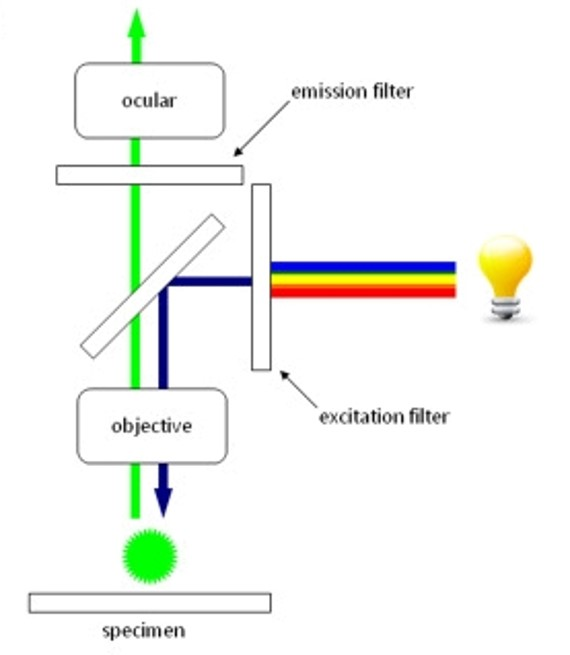
\includegraphics[width=0.5\textwidth]{epi.jpg}
\caption{Epifluoreszcens mikroszkóp sematikus rajza}
\label{epi}
\end{figure}
A fényforrás epifluoreszcens mikroszkópokban a gerjesztésre időben valamint a látható tartományban folytonos spektrumú fényforrás használatos ami esetünkben higanygőz lámpa. Ezután a kiválasztjuk a fluorofórnak megfelelő hullámhosszat az úgynevezett gerjesztési szűrővel. Ezután a fény egy dikroikus tükrön visszaverődve valamint az objektíven keresztül a mintára esik, majd a fluoreszcens jel ugyanezen objektíven és ezúttal a dikroikus tükrön is áthaladva egy további, emissziós szűrőre esik majd utána egy detektorra. Érdemes lehet alkalmazunk dikroikus tükröket és szűrőket egyszerre, noha ezek külön-külön is szűrik a jelet, érdemes lehet a lehető leginkább elkülöníteni a gerjesztő- és válaszjelet mivel a gerjesztés intenzitása akár nagyságrendekkel nagyobb ezért kis áthatolás esetén is ronthatja a kapott képet.
\subsection{Felvétel készítése}
Az általunk használt mikroszkóp váz típusa Nikon Ti/2 Eclipse volt. Ezen 20-szoros nagyítású objektívet használtunk, a kamera egy 2048$\times$2048 pixel felbontású kamera volt, megvilágításra higanygőz lámpát használtunk. A minta 3 színnel volt megfestve, egy narancssárga, zöld és kék fény által gerjesztett festékkel. A képen az egyes színek a hozzájuk tartozó festéket reprezentálja. 
\begin{figure}[H]
\centering
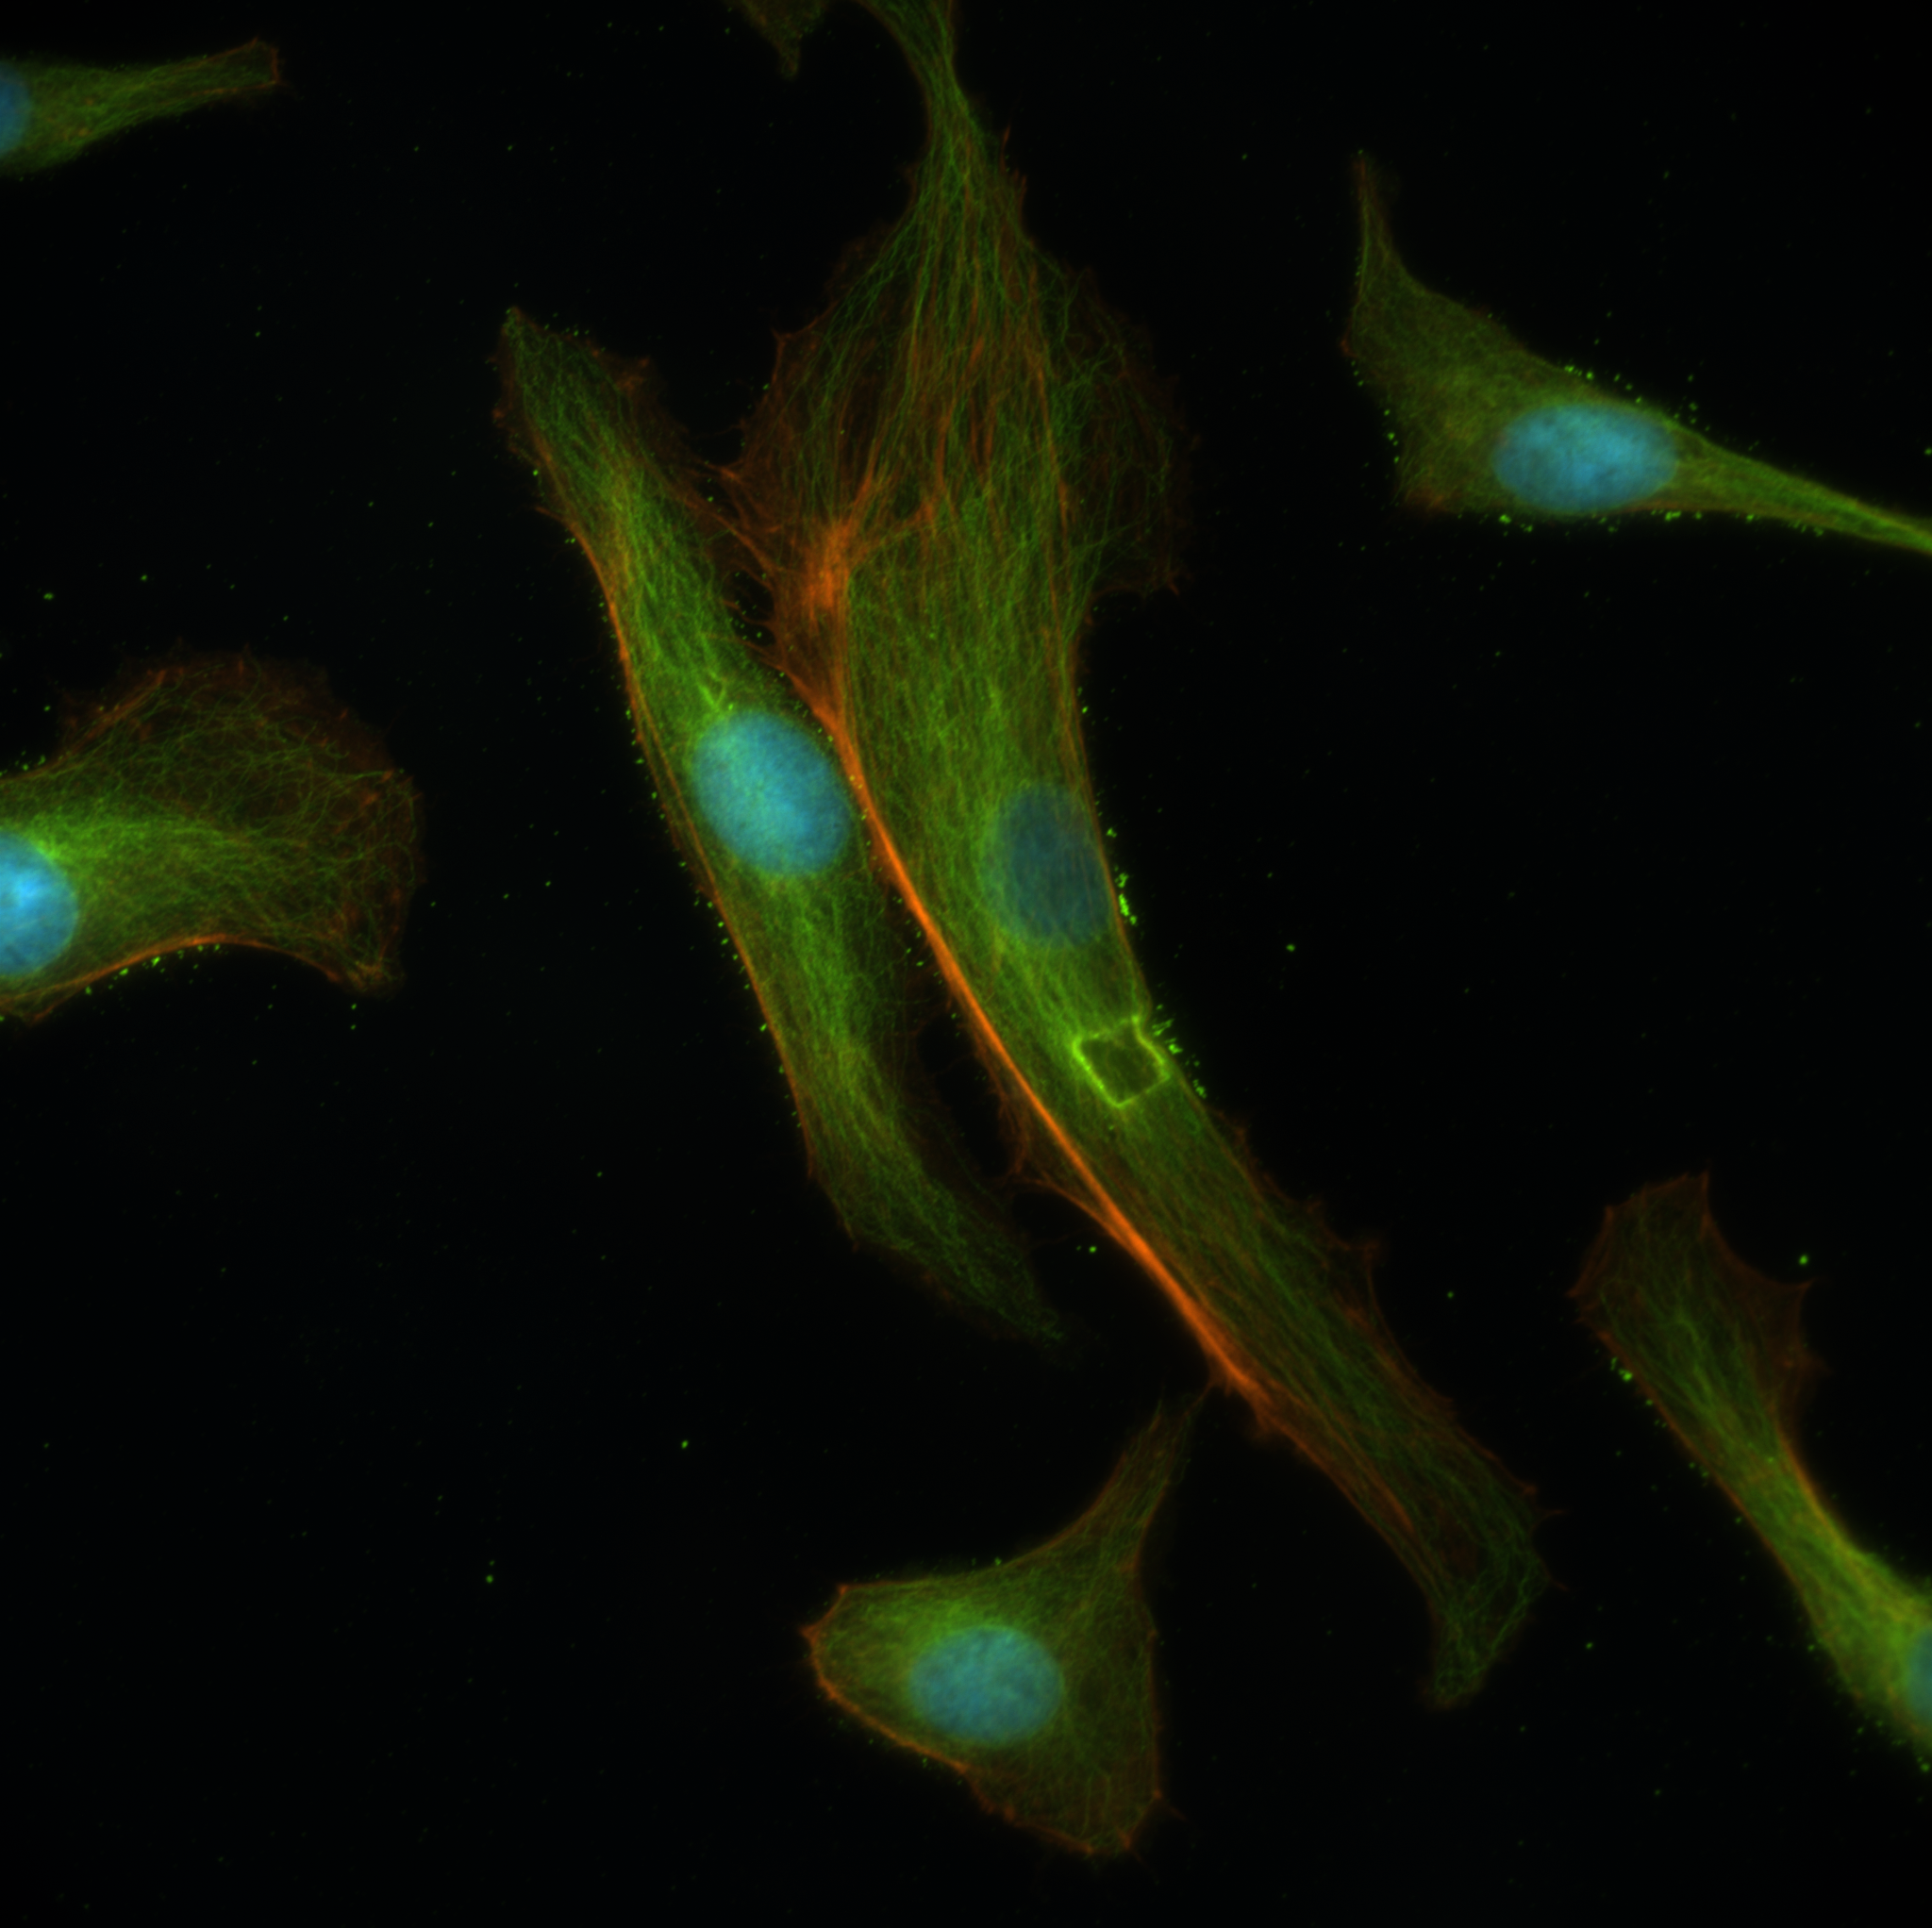
\includegraphics[width=0.75\textwidth]{./Confocal/Epi.png}
\caption{Epifluoreszcens kompozit kép}
\end{figure}
A képen szépen látható a sejt felépítése, jól elkülönül a kék sejtmag, a zöld belső hálós szerkezet és a narancs külső háló. A szerkezet további vizsgálata érdekében válasszuk szét az egyes felvételeket.
\begin{figure}[H]
\centering
\begin{subfigure}{0.32\textwidth}
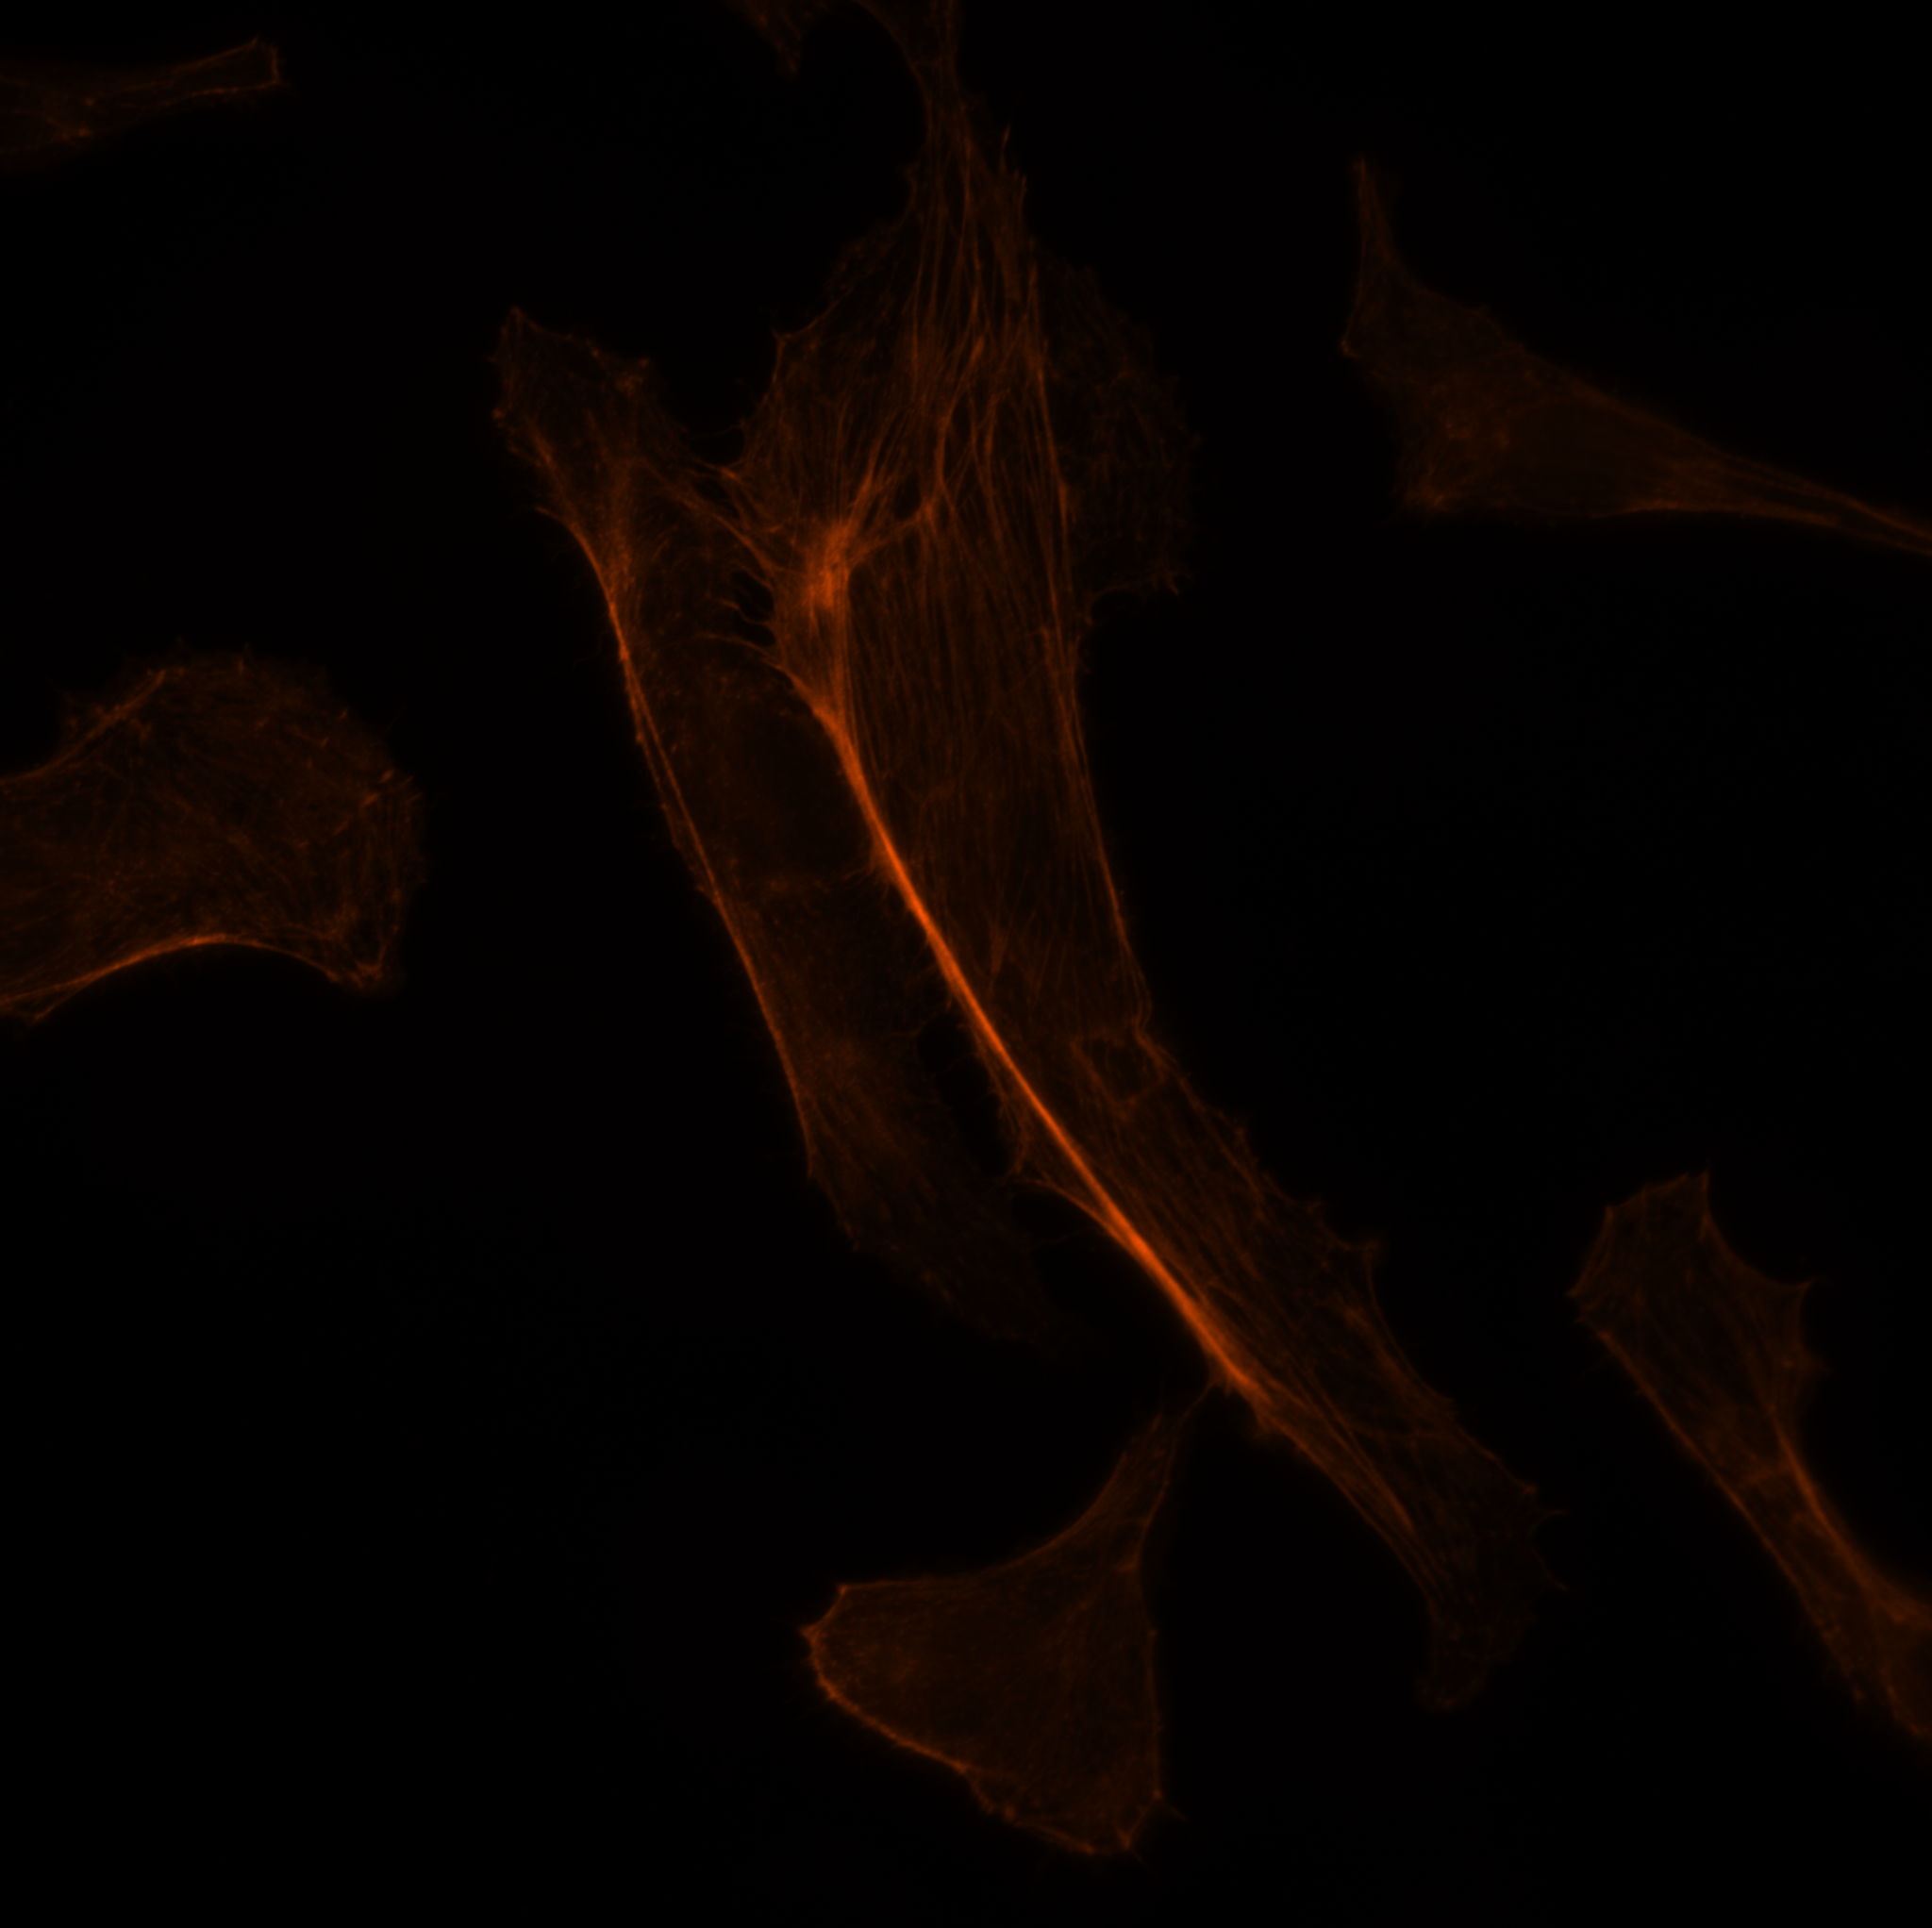
\includegraphics[width=\textwidth]{./Confocal/pEpi.png}
\end{subfigure}
\begin{subfigure}{0.32\textwidth}
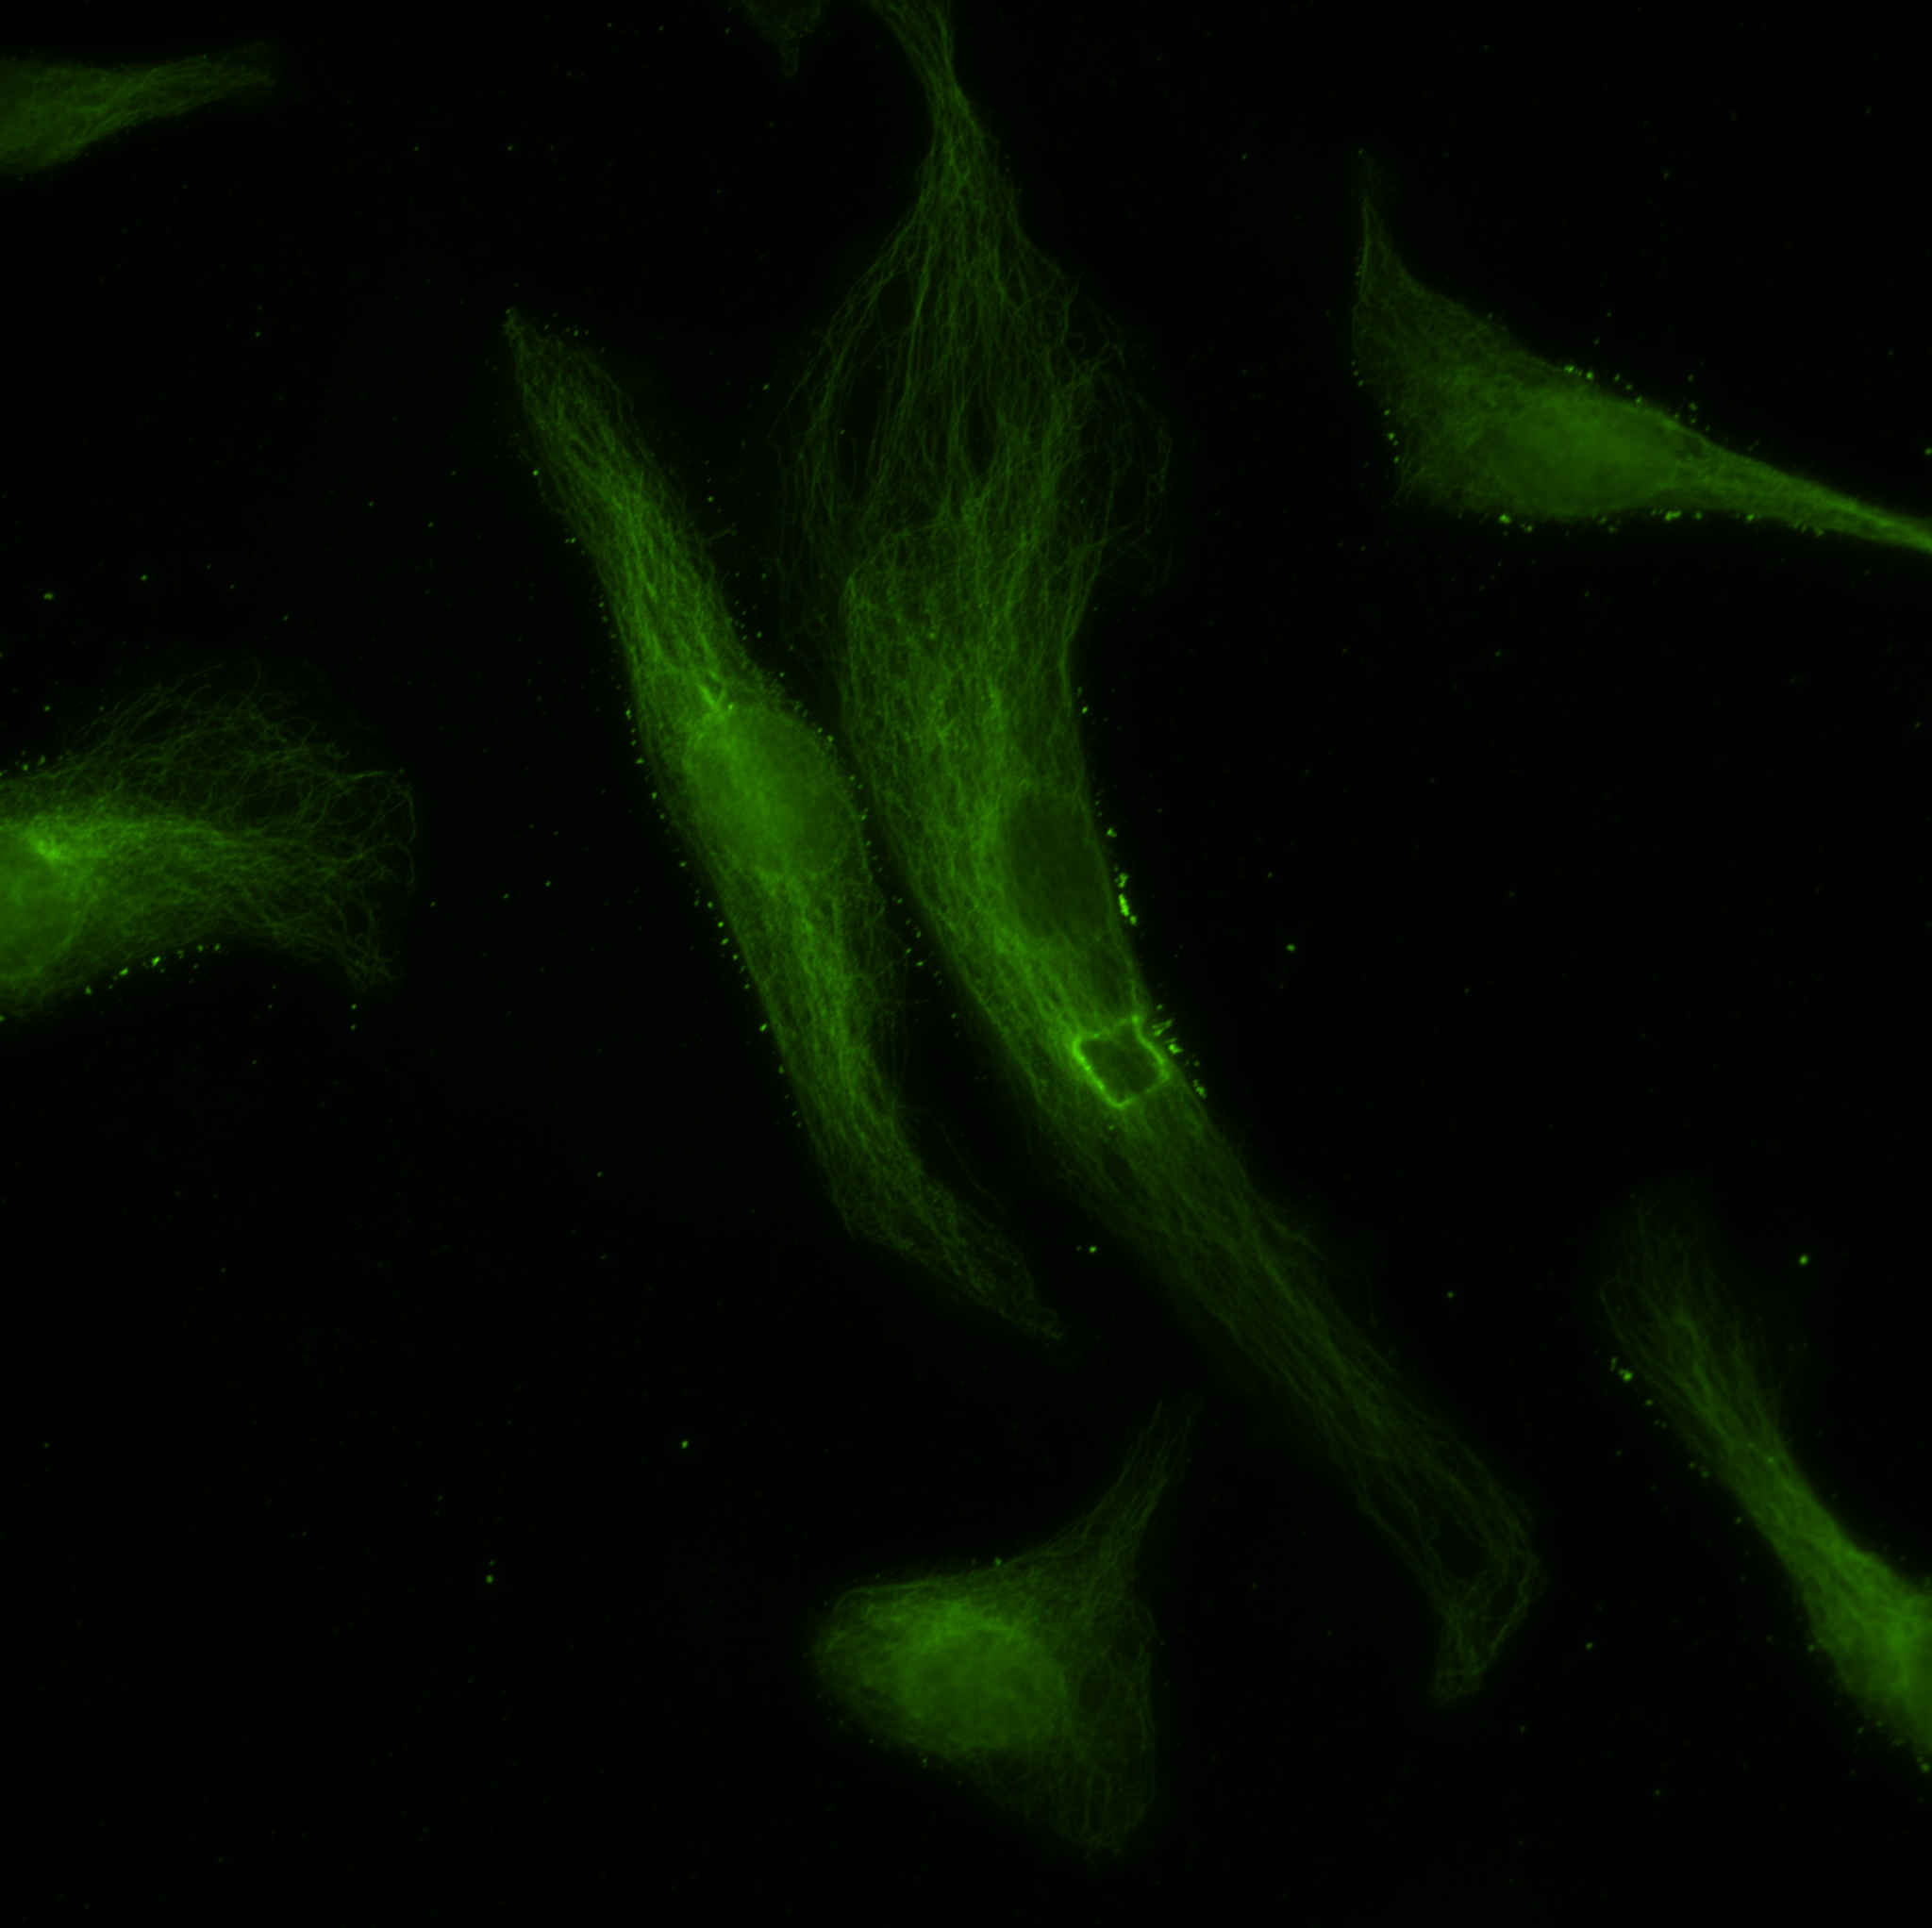
\includegraphics[width=\textwidth]{./Confocal/zEpi.png}
\end{subfigure}
\begin{subfigure}{0.32\textwidth}
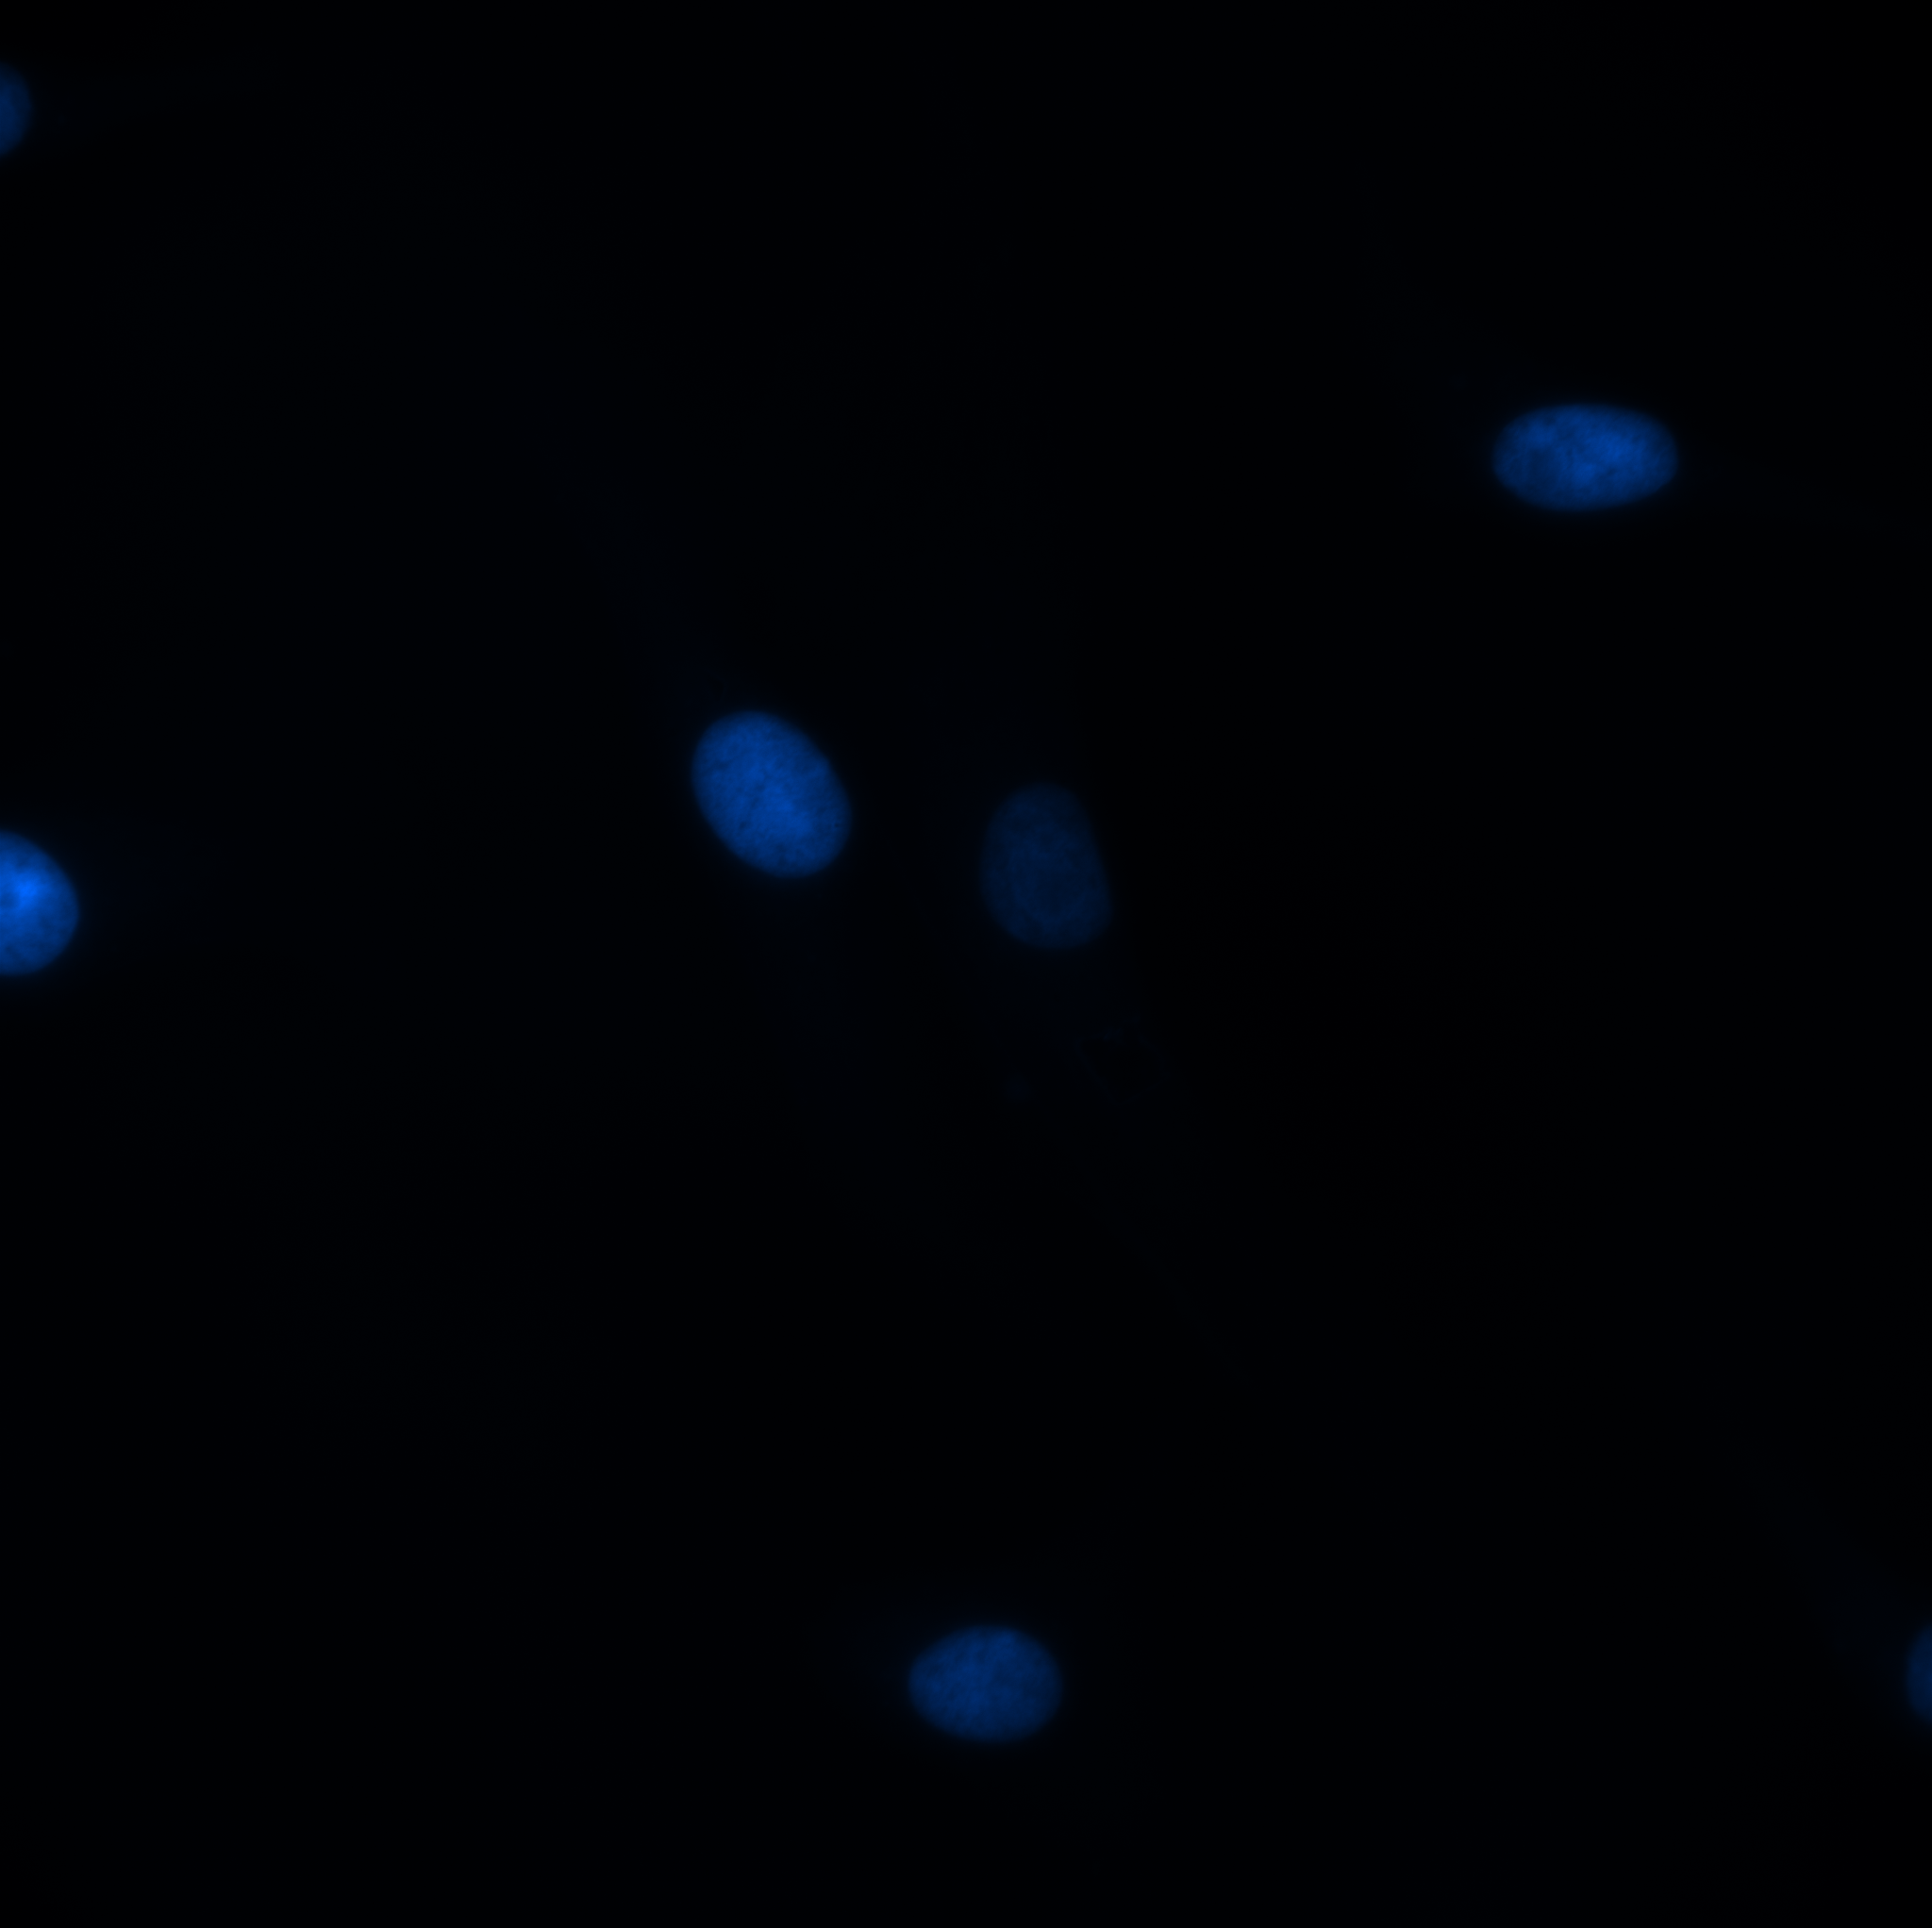
\includegraphics[width=\textwidth]{./Confocal/kEpi.png}
\end{subfigure}
\caption{Epifluoreszcens csatornák elkülönítve}
\end{figure}
Az elkülönített és összeillesztett képeket együtt vizsgálva jól láthatjuk a minta felépítését, azonban a felbontás tovább javítható, valamint további információ nyerhető ki akkor, ha a mintát megvizsgáljuk konfogkális üzemmódban.
\section{Konfokális mikroszkópia}
\subsection{Elmélet áttekintés}
A konfokális mikroszkóp az epifloureszcens mikroszkóp egy továbbfejlesztett változata.
\end{document}